\documentclass[9pt]{article}
\usepackage[utf8]{inputenc}
\usepackage{amsmath,amsthm,amsfonts,amssymb,amscd}
\usepackage{multirow,booktabs}
\usepackage{enumitem}
\usepackage{fancyhdr}
\usepackage{mathrsfs}
\usepackage{wrapfig}
\usepackage{setspace}
\usepackage{calc}
\usepackage{multicol}
\usepackage{cancel}
\usepackage[retainorgcmds]{IEEEtrantools}
\usepackage{framed}
\usepackage[most]{tcolorbox}
\usepackage{tikz}
\usepackage{geometry}
\geometry{
	a4paper,
	total={170mm,257mm},
	left=20mm,
	top=20mm,
}
\title{Electromagnetic Induction}
\author{Aaron G.K.}
\begin{document}
	\maketitle
	\section*{Faraday's Law}
	In nature, we often observe symmetry whenever we carefully look for it. Especially in physics, some important hypotheses were a result of the assumption that many phenomena might be symmetric. So far, we have seen a lot of electromagnetic effects such as Ampere's Law and the Motor Effect. What these effects have in common is that magnetic fields are induced as a result of current. Now, we are about to see the reverse process- the generation of current from magnetic field. This was first observed independently by Joseph Henry \& Michael Faraday a little over a decade after Oersted's revolutionary discovery. Their experiments were rather simple.
	\begin{center}
		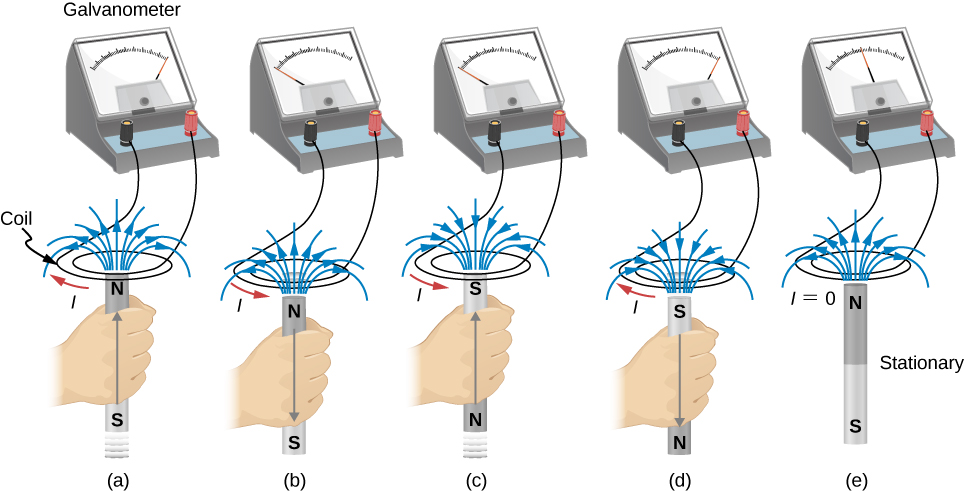
\includegraphics[scale=0.6]{FaradayExp}
	\end{center}
	One of the first experiments concerning the effects of time-varying magnetic fields were performed by Michael Faraday in early 19th century. A variation of the experiment is shown in the figure above. An emf is induced when the magnetic field in the coil is changed by pushing a bar magnet into or out of the coil. Emfs of opposite signs are produced by motion in opposite directions, and the directions of emfs are also reversed by reversing poles. The same results are produced if the coil is moved rather than the magnet—it is the relative motion that is important. The faster the motion, the greater the emf, and there is no emf when the magnet is stationary relative to the coil. \\ \\
	The key observation by Faraday is that in both experiments, a current flowed in the circuit only when the magnetic field in the region occupied by that circuit \textbf{was changing}. As the magnet of the figure was moved, the strength of its magnetic field at the loop changed. Faraday was eventually able to interpret these and all other experiments involving magnetic fields that vary with time in terms of the following law named after him. It states that: \\ \\
	\textit{The emf $\varepsilon$ induced is the negative change in the magnetic flux  $\Phi_m$ per unit time. Any change in the magnetic field or change in orientation of the area of the coil with respect to the magnetic field induces a voltage (emf).} 
	\subsection*{Magnetic Flux}
	The magnetic flux is a measurement of the amount of magnetic field lines through a given surface area as shown below:
	\begin{center}
		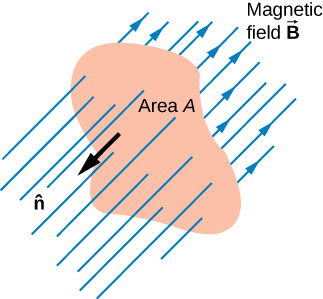
\includegraphics[scale=0.6]{flux_area}
	\end{center}
	If the angle between the unit area $\hat{A}$ and magnetic field vector $\vec{B}$ are parallel or antiparallel, as shown in the diagram, the magnetic flux is the highest possible value given the values of area and magnetic field. Bearing that in mind, we can simply express the flux as follows:
	$$\Phi_m=B_\perp A$$
	\begin{center}
		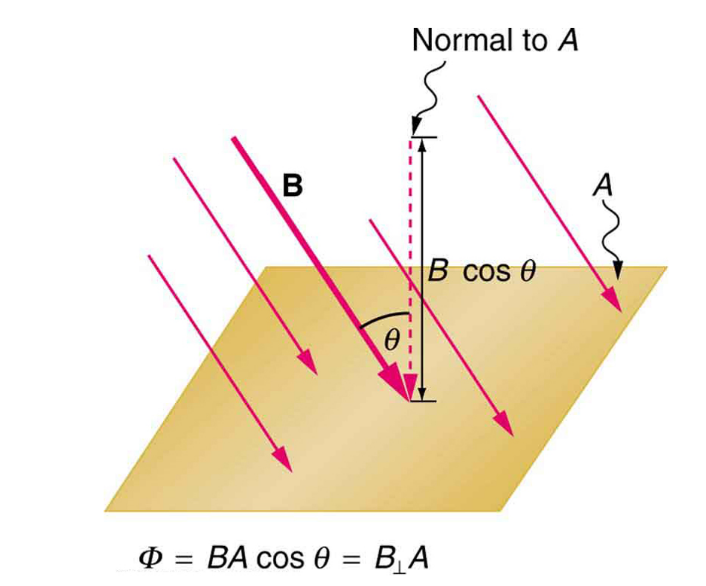
\includegraphics[scale=0.18]{flux}
	\end{center}
	Area Vector($\vec{A}$) - is a vector of a planar surface whose magnitude is equal to the area of the surface and its direction is perpendicular to the surface. We express the direction of the Area vector with the unit vector $\hat{A}$ or $\hat{n}$. \\ \\
	On the other hand, we can express the magnetic field strength in terms of the flux and area as follows which earns the magnetic field strength the name \textit{magnetic flux density}.
	$$B_\perp=\dfrac{\Phi_m}{A}$$
	Going back to flux, we can see that the SI unit of this so-called flux is $Tm^2$ and it is called \textit{Weber(Wb)}. Flux can generally be described as the dot product between the magnetic field strength and the area vector.
	$$\Phi_m=\vec{B}\cdot\vec{A}$$
	Consequently, the flux can be expressed as
	$$\Phi_m=BA\cos\theta\text{, such that }\theta\text{ is the angle between the area vector and magnetic field.}$$
	When Michael Faraday was doing experiments involving induction of current from magnetic he noticed one important thing: current only arose when the flux was changing - not necessarily the magnetic field. There are many ways we can change the flux including by
	\begin{itemize}
		\item changing the magnetic field ($\vec{B}$)
		\item changing the area of the loop ($\vec{A}$)
		\item changing the relative orientation of the system and field ($\theta$)
	\end{itemize}
	Let's consider a a loop of a conductor in a magnetic field, the easiest out of all the three quantities to change is obviously the orientation of the wire along the field. We can rotate the loop and each time, we can keep changing the orientation at each instant and hence have the flux changing to generate EMF. Think of hydroelectric power plants for instance. You have probably heard about having a lot of water in the reservoir and releasing it at a pace to rotate turbines which in turn generate electricity. This rotation of turbines causes changes in the flux which in turn causes EMF to generate. This is Faraday's law in a nutshell.\\ \\
	As we have briefly seen above, \textbf{Faraday's Law} states that the magnitude of the induced EMF is proportional to the time rate of the change in flux. Mathematically,
	$$\varepsilon\propto\dfrac{\Delta\Phi}{\Delta t}$$
	Faraday's law tells us about the magnitude of the induced EMF. However, the direction of the induced EMF is given by a law called Lenz's Law, that is based on the conservation of energy.
	\subsection*{Lenz's Law}
	\textbf{Lenz's law} tells us that \textit{the direction of the induced current is such as to oppose the change causing it}. If the cause is an increase in flux, the induced current acts to decrease the flux. If the cause is a decrease in flux, the induced current acts to increase the flux. \\ \\
	Lenz’s law can be considered in terms of conservation of energy. If pushing a magnet into a coil causes current, the energy in that current must have come from somewhere(\textit{the push}). If the induced current causes a magnetic field opposing the increase in field of the magnet we pushed in, then the situation is clear because we pushed a magnet against a field and did work on the system, and that showed up as current. If it were not the case that the induced field opposes the change in the flux, the magnet would be pulled in produce a current without anything having done work which means Electric potential energy would have been created, violating the conservation of energy.  We can also explain it in terms of Newton's Third Law: magnetic force is created in action and reaction pairs during induction.\\ \\
	To understand this law, let's consider the following situations below:
	\begin{center}
		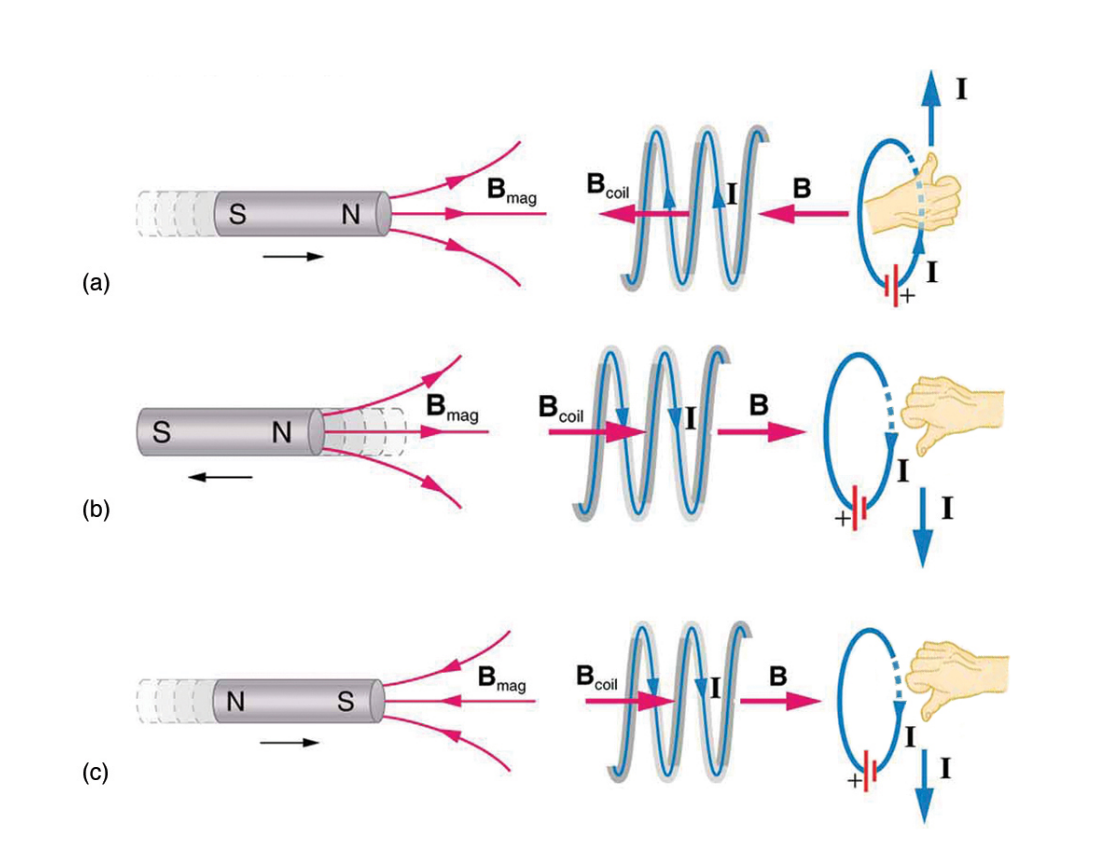
\includegraphics[scale=0.25]{lenzs_law}
	\end{center}
	In \textbf{(a)}, the north pole of a magnet is approaching the coil of wire and since the flux is changing, EMF is being induced. We can deduce the magnitude of the EMF being induced using Faraday's law. However, to determine the direction of the induced current, we use Lenz's law. Since the north pole of the magnet is approaching the coil, Lenz's law tells us that the direction the induced current acts so as to oppose the change causing it(the change is the North pole approaching the coil). Thus, the induced current will create a magnetic field that would oppose the applied magnetic field. In that case, the magnetic field by the induced current is going to be a North pole on the left side of the loop to oppose the motion of the magnet causing the induction. Then, we can use the Right Hand Rule to see the direction of the current that causes such a magnetic field. \newline\newline
	In case \textbf{(b)}, the north pole of the magnet is moving away from the coil of wire, thus the to oppose this change, the magnetic field by the induced current at the end of the coil by the magnet should be the south pole. Thus, we can use the Right Hand Rule to determine which direction of the current will induce such an orientation of magnetic field on the solenoid.\newline\newline
	Thus, we can generalize the dynamo effect in the following equation(considering there are N loops of wire getting crossed by the magnetic field):
	$$\varepsilon=-\text{N}\dfrac{\Delta\Phi_m}{\Delta t}$$
	The negative sign addition we have here is to signify that the EMF generated will have an opposing effect to the change causing the induction.
	\section*{Inductance}
	\begin{center}
		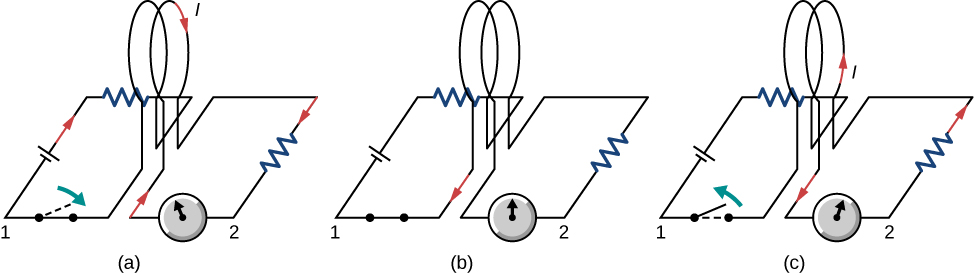
\includegraphics[scale=0.8]{faraday_ind}
	\end{center}
	Faraday also discovered that a current could be induced using two circuits without a presence of a magnet — a changing current in one circuit induces a current in a second, nearby circuit. For example, when the switch is closed in circuit 1 of the figure above, the ammeter needle of circuit 2 momentarily deflects, indicating that a short-lived current surge has been induced in that circuit. The ammeter needle quickly returns to its original position, where it remains. However, if the switch of circuit 1 is now suddenly opened, another short-lived current surge in the direction opposite from before is observed in circuit 2. \\ \\
	Similar to the simple experiment in induction, closing the switch of circuit 1 produces a short-lived current surge in circuit 2. However, if the switch remains closed, no current is observed in circuit 2. Opening the switch again produces a short-lived current in circuit 2 but in the opposite direction from before. This shows that, similar to the phenomenon we saw in induction, the flux needs to be changing for current to be induced.
	\subsection*{Mutual-inductance}
	Mutual inductance, similar to self-inductance is the generation of current on another device due to the change in current in one device. It is the effect of Faraday's law. As the current in one device changes, the magnetic fluxes due to the current changes and hence nearby conductors will experience a flux change through them and that will induce EMF. We can determine the direction of the induced current using Lenz's law and the magnitude of the induced EMF is proportional to the change in current.
	$$\varepsilon\propto\dfrac{\varDelta I}{\varDelta t}$$
	$$\varepsilon=-\text{M}\dfrac{\varDelta I}{\varDelta t}$$
	\textbf{M} is called the mutual-inductance of a given conductor and it is the measure of the effectiveness of inductance of current.
	\subsection*{Self-inductance}
	When current is changing through a conductor, we can see the effect of Faraday's law on it. We know that when current is flowing through a conductor, there is a magnetic field. And when the current changes, there will be a change in the magnetic field and as a result, there will be a change in magnetic flux and hence, current will be induced. This phenomenon is called \textbf{self-inductance} and we can explain it using Lenz's law. The induced EMF is proportional to the time rate of change in the current:
	$$\varepsilon\propto\dfrac{\Delta I}{\Delta t}$$
	The constant of proportionality for the above relationship is called self-inductance(\textbf{L}), thus we have the following:
	$$\varepsilon=-\text{L}\dfrac{\Delta I}{\Delta t}$$
	\begin{itemize}
		\item The negative sign on here is also a result of Lenz's law. It tells us that the EMF that is induced opposes the change in current.
		\item The SI unit of self-inductance is Henry(H). \textit{Do you remember that the SI unit of permeability was} H/m?
	\end{itemize}
	Self-inductance implies opposition to change in current, this implies that for a conductor with a large self-inductance, it is hard to achieve change in current quickly.
	\subsubsection*{Self-inductance of a solenoid}
	We have seen that self-inductance is given by:
	$$\varepsilon=-\text{L}\dfrac{\Delta I}{\Delta t}$$
	We also know that the EMF given by the dynamo effect is given by:
	$$\varepsilon=-\text{N}\dfrac{\Delta\phi}{\Delta t}$$
	When we combine the above two equations together, we get, 
	$$-\text{N}\dfrac{\Delta\phi}{\Delta t}=-\text{L}\dfrac{\Delta I}{\Delta t }$$
	We see that the self-inductance(L) is given by:
	$$L=N\dfrac{\Delta\phi}{\Delta I}$$
	We know that for a solenoid, the magnetic flux density is given by:
	$$\textbf{B}=\mu_0nI$$
	$$L=N\dfrac{\Delta BA}{\Delta t}=N\dfrac{\Delta (\mu_0nI)A}{\Delta I}$$
	Since $n=\dfrac{N}{L}$, we have:
	$$\text{L}=\dfrac{\mu_0N^2A}{L}$$
	\subsection*{Transformers}
	Transformers work using the concept of mutual inductance. As the name indicates, they transform voltage from one value to another. Power is sent long distances at high voltages, because less current is required for a given amount of
	power. But high voltages pose greater hazards, so transformers are employed to produce lower voltage at the user’s location. Based on the amount of the output voltage we categorize transformers into step-up and step-down which amplify and decrease the voltage respectively.
	\begin{center}
		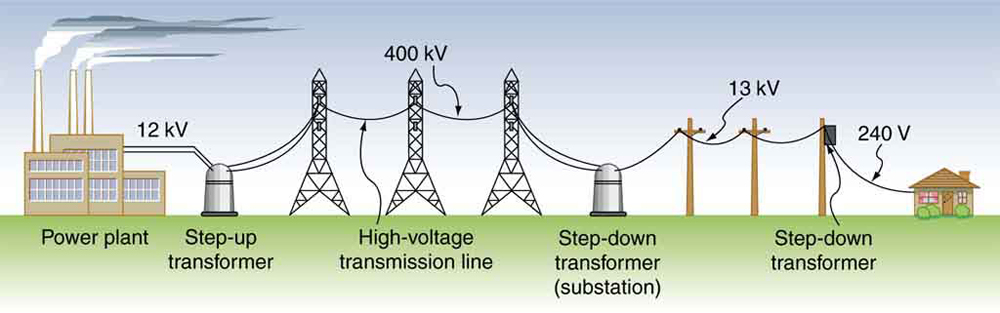
\includegraphics[scale=0.5]{transformers}
	\end{center}
	Let's consider the transformer below, for instance:
	\begin{center}
		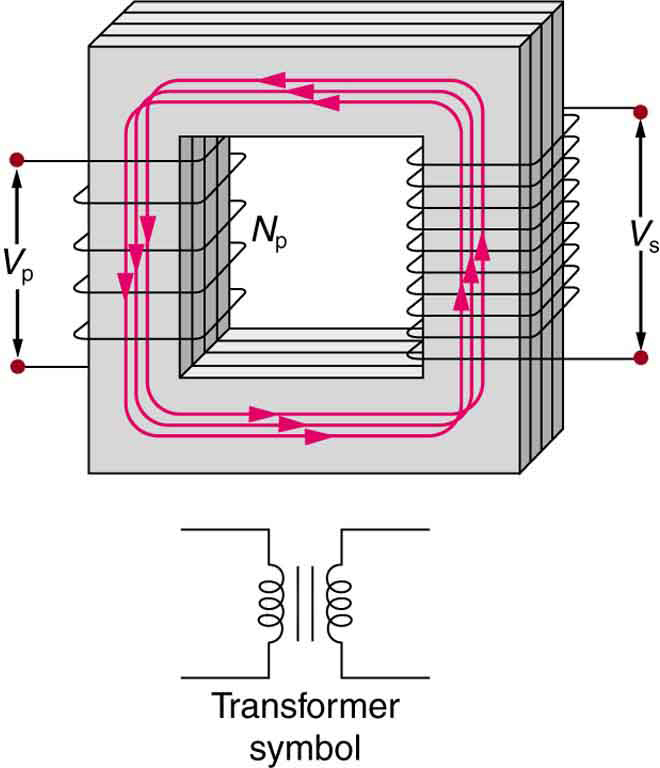
\includegraphics[scale=0.35]{transformer}
	\end{center}
	For a simple transformer such as the one shown above, the output voltage depends almost entirely on the input voltage and the ratio of the number of loops in the primary and secondary coils. Faraday’s law of induction for the secondary coil gives its induced output voltage to be:
	$$V_s=-\text{N}_\text{s}\dfrac{\Delta\phi}{\Delta t}$$
	Since the rate of change in flux is the same for each case, we have the following equation(the \textbf{Transformer Equation}) be true:
	$$\dfrac{V_s}{N_s}=\dfrac{V_p}{N_p}\iff\dfrac{V_s}{V_p}=\dfrac{N_s}{N_p}$$
	Since power is conserved, the input power(primary) of the transformer should equal the output(secondary) in ideal cases.
	$$P_{p}=P_{s}$$
	$$V_pI_p=V_sI_s$$
	$$\dfrac{V_p}{I_s}=\dfrac{V_s}{I_p}$$
	Thus, we can see that whenever we have a step-up transformer, the current is bound to decrease while in a step-down transformer, the current increases.
	\subsection*{Motional EMF}
	Whenever flux is changing through a conductor, EMF is induced. We have seen when discussing Dynamo Effect that flux change occurs as a result of relative motion between the source of magnetic field and the conductor. In this specific case, we will look at the case in which the conductor is moving.
	\begin{center}
		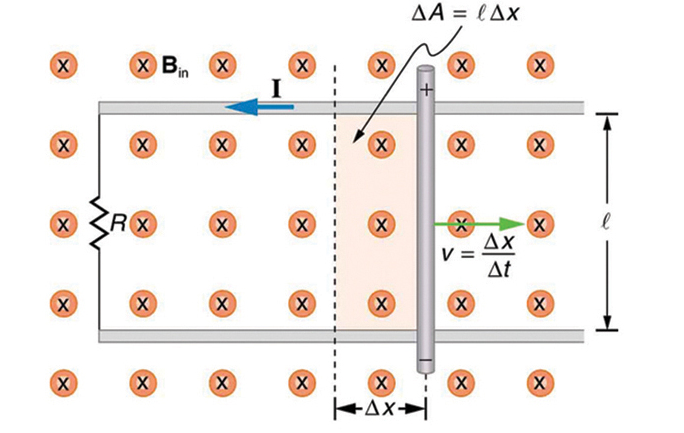
\includegraphics[scale=0.5]{motional_EMF}
	\end{center}
	We have seen one case of motional EMF early on in this unit when discussing the Hall Effect. Consider a conductor moving through a magnetic field as shown in the figure above. As the conductor is moving through the field, EMF is induced according to Faraday's law:
	$$\varepsilon=-N\dfrac{\Delta\phi}{\varDelta t}$$
	$$\varepsilon=-N\dfrac{\Delta BA}{\varDelta t}$$
	$$\varepsilon=-N\dfrac{ Bl\Delta x}{\Delta t}\text{, but }\dfrac{\Delta x}{\Delta t}=v$$
	$$\varepsilon=-N\dfrac{ Bl\Delta x}{\Delta t}$$
	$$\varepsilon=-NBlv$$
	For the simplest case, $N=1$, thus
	$$\varepsilon=-Blv$$
	However, we see that the induced EMF is perpendicular to both the velocity and the magnetic field.
\end{document}	